\documentclass[border=10pt]{standalone}

\usepackage{tikz}
\usepackage{tikzsymbols}
\usetikzlibrary{calc,patterns,shapes.geometric}

\def\centerarc[#1](#2)(#3:#4:#5){\draw[#1] ($(#2)+({#5*cos(#3)},{#5*sin(#3)})$) arc (#3:#4:#5);}

\begin{document}
	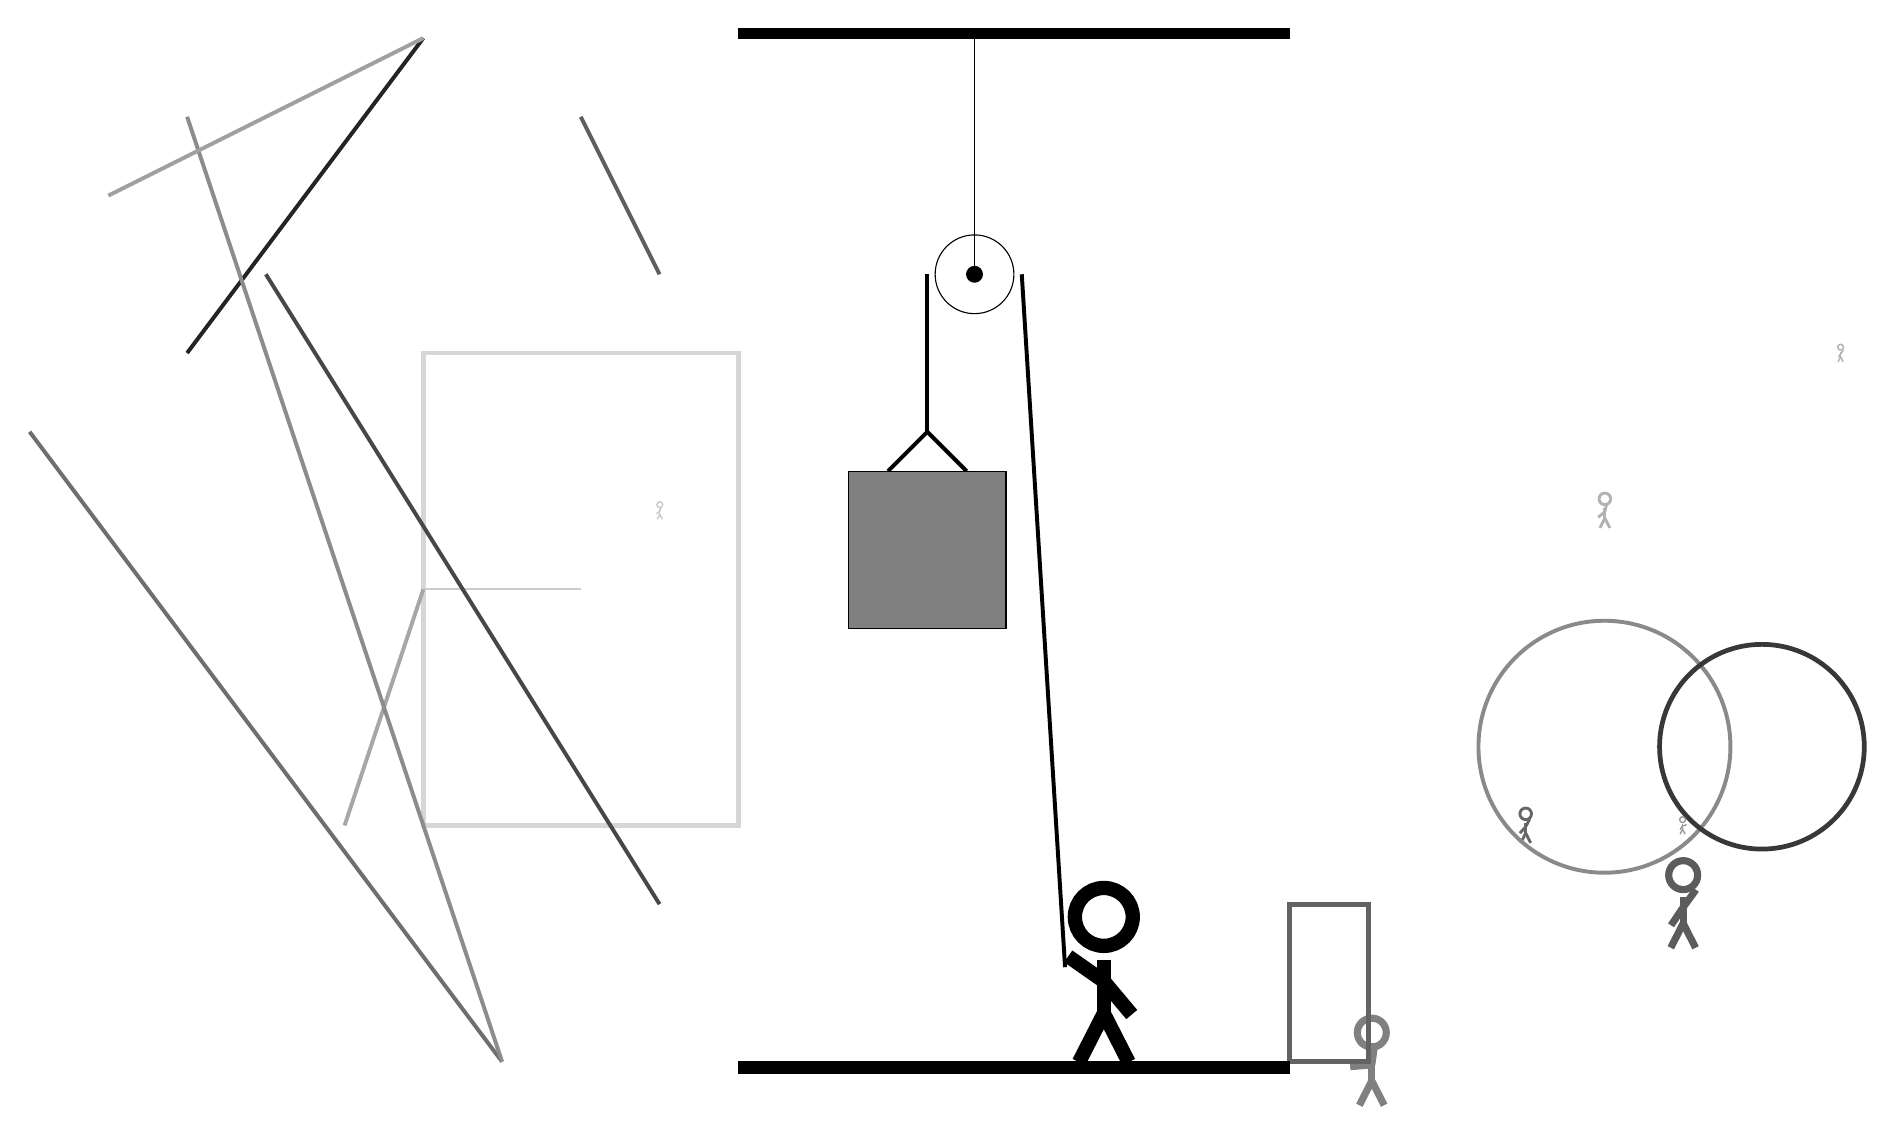
\begin{tikzpicture}
		%%%%% START %%%%%
		
		\draw[fill=black] (-2, 10) rectangle (5, 10.125);
		
		\draw (1, 7) circle (0.5);
		\draw[fill=black] (1, 7) circle (0.1);
		\draw (1, 10) -- (1, 7);
		
		\draw[line width=0.6mm, color=black!67] (7, 6) rectangle (7, 6);
		
		\draw[line width=0.6mm, color=black!16] (-2, 6) rectangle (-6, 0);
		\draw[line width=0.5mm, color=black!57](-5, -3) -- (-11, 5);
		\draw[line width=0.5mm, color=black!86](-6, 10) -- (-9, 6);
		\draw[line width=0.5mm, color=black!35](-7, 0) -- (-6, 3);
		\draw[line width=0.3mm, color=black!20] (-4, 3) rectangle (-6, 3);
		\node[line width=0.7mm, color=black!50] at (6, -3) {\Strichmaxerl[5][5][82]};
		
		\node[line width=0.7mm, color=black!21] at (-3, 4) {\Strichmaxerl[1][40][75]};
		\draw[line width=0.5mm, color=black!45](-5, -3) -- (-9, 9);
		\node[line width=0.6mm, color=black!64] at (10, -1) {\Strichmaxerl[5][56][54]};
		\node[line width=0.6mm, color=black!30] at (9, 4) {\Strichmaxerl[2][40][77]};
		
		\node[line width=0.3mm, color=black!60] at (8, 0) {\Strichmaxerl[2][48][62]};
		\node[line width=0.4mm, color=black!31] at (12, 6) {\Strichmaxerl[1][59][51]};
		
		\draw [line width=0.5mm, color=black!46](9, 1) circle (1.6);
		\draw[line width=0.5mm, color=black!37](-6, 10) -- (-10, 8);
		\draw [line width=0.6mm, color=black!78](11, 1) circle (1.3);
		
		\draw[line width=0.5mm, color=black!72](-3, -1) -- (-8, 7);
		\node[line width=0.2mm, color=black!40] at (10, 0) {\Strichmaxerl[1][54][19]};
		\draw[line width=0.5mm, color=black!63](-4, 9) -- (-3, 7);
		\draw[line width=0.6mm, color=black!61] (6, -1) rectangle (5, -3);
		
		\draw[line width=0.5mm] (-0.1, 4.5) -- (0.4, 5.0) -- (0.9, 4.5);
		\draw[fill=black!50] (-0.6, 4.5) rectangle (1.4, 2.5);
		
		\draw[line width=0.5mm] (0.4, 7) -- (0.4, 5.0);
		\centerarc[line width=0.5mm](1, 7)(0:180:0.6);
		\draw[line width=0.5mm](1.6, 7) -- (2.15, -1.8);
		
		\node at (2.6, -1.9) {\Strichmaxerl[10][-35][-50]};
		
		\draw[fill=black] (-2, -3) rectangle (5, -3.15);
		
		%%%%% END %%%%%
	\end{tikzpicture}
\end{document}